\documentclass[a4paper,12pt]{article}

\usepackage[russian]{babel} % Язык документа

% Подключаем fontspec для управления шрифтами
\usepackage{fontspec}

% Выбираем шрифты с поддержкой кириллицы (установленные в системе)
\setmainfont{CMU Serif} % или "Times New Roman", или "Linux Libertine O"
\setsansfont{CMU Sans Serif}
\setmonofont{CMU Typewriter Text}

\usepackage{geometry}
\geometry{left=30mm, right=10mm, top=20mm, bottom=20mm}

\usepackage{setspace}
\onehalfspacing
\setlength{\parindent}{15mm}

\usepackage{graphicx}
\usepackage{caption}
\usepackage{booktabs}
\usepackage{amsmath}
\usepackage{tocloft}
\usepackage{titlesec}
\usepackage{float}
\usepackage{hyperref}
\usepackage{listings}
\usepackage{xcolor}

\lstset{
	language=Python,
	basicstyle=\ttfamily\small,
	keywordstyle=\color{blue}\bfseries,
	stringstyle=\color{red},
	commentstyle=\color{green!50!black},
	numbers=left,
	numberstyle=\tiny,
	stepnumber=1,
	numbersep=5pt,
	showspaces=false,
	showstringspaces=false,
	frame=none,
	breaklines=true,
	breakatwhitespace=true,
	tabsize=2,
	columns=fullflexible,
	mathescape=false,
}

\titleformat{\section}{\normalfont\bfseries}{\thesection}{1em}{}
\titleformat{\subsection}{\normalfont\bfseries}{\thesubsection}{1em}{}

% Форматирование титульной страницы
\begin{document}

\begin{titlepage}
	\vspace*{1cm}
	{\small
		\begin{center}
			МИНИСТЕРСТВО НАУКИ И ВЫСШЕГО ОБРАЗОВАНИЯ РОССИЙСКОЙ ФЕДЕРАЦИИ\\
			ФЕДЕРАЛЬНОЕ ГОСУДАРСТВЕННОЕ АВТОНОМНОЕ ОБРАЗОВАТЕЛЬНОЕ УЧРЕЖДЕНИЕ ВЫСШЕГО ОБРАЗОВАНИЯ\\
			\textbf{НАЦИОНАЛЬНЫЙ ИССЛЕДОВАТЕЛЬСКИЙ ТОМСКИЙ ПОЛИТЕХНИЧЕСКИЙ УНИВЕРСИТЕТ}
		\end{center}
	}
	\vspace{0.5cm}
	\begin{center}
		Инженерная школа информационных технологий и робототехники\\
		Отделение информационных технологий\\
		Направление: 09.04.01 Искусственный интеллект и машинное обучение
	\end{center}
	\vspace{1cm}
	\begin{center}
		\textbf{ОТЧЁТ ПО ПРАКТИЧЕСКОЙ РАБОТЕ}
	\end{center}
	\begin{center}
		по дисциплине: Нейроэволюционные вычисления
	\end{center}
	\vspace{0.5cm}
	\begin{center}
		\textbf{Вариант 6}
	\end{center}
	\begin{center}
		на тему: Эволюционное обучение однослойной нейросети методом HESP на задаче посадки космического аппарата
	\end{center}
	\vspace{1cm}
	
	% Двухколоночное расположение
	\begin{tabular}{p{0.3\textwidth} p{0.35\textwidth} p{0.3\textwidth}}
		\textbf{Выполнил:} & студент гр. 8ВМ42 \newline Волков Д.А. & 10.06.2025 \\
		& & \\
		\textbf{Проверил:} & к.т.н., Доцент ОИТ ИШИТР \newline Григорьев Д.С. & 10.06.2025
	\end{tabular}
	\vfill
	\begin{center}
		Томск – 2025
	\end{center}
\end{titlepage}


% Оглавление
\tableofcontents
\setcounter{page}{2}
\newpage

% Настройка форматирования разделов и интервалов
\titleformat{\section}{\normalfont\bfseries}{\thesection}{1em}{}
\titleformat{\subsection}{\normalfont\bfseries}{\thesubsection}{1em}{}
\setlength{\parindent}{15mm}
\onehalfspacing

% Раздел 1: Введение
\section{Введение}

Нейроэволюционные подходы играют всё более значимую роль в современном машинном обучении, особенно в задачах, где традиционные методы, такие как градиентный спуск и обратное распространение ошибки, оказываются неприменимыми или неэффективными. Эти методы вдохновлены процессами естественного отбора и направлены на эволюционное развитие популяций агентов или их составляющих с целью повышения приспособленности к решаемой задаче. 

Одним из продвинутых нейроэволюционных алгоритмов является HESP (Hierarchical Evolution of Subpopulations), предлагающий более гибкий подход к эволюции нейронных сетей за счёт иерархической структуры и коэволюции отдельных нейронов, а не целых особей. 
Такой подход позволяет сохранять локально успешные особенности поведения и эффективно использовать их в процессе формирования новых конфигураций сети.

HESP хорошо подходит для задач непрерывного управления, таких как посадка лунного модуля в среде \texttt{LunarLanderContinuous-v3} библиотеки Gymnasium. Эта задача требует от агента принятия непрерывных решений в реальном времени на основе текущего состояния среды, таких как положение, скорость и угол наклона. Агент должен обеспечить мягкую посадку, контролируя основной и боковые двигатели при минимальных затратах топлива и без столкновений с поверхностью.

В данной работе была реализована однослойная нейронная сеть, обучаемая с помощью алгоритма HESP без использования сторонних библиотек. Особенностью подхода является акцент на визуализации топологии сети, а также построение графиков, отражающих динамику обучения. Процесс обучения включал сохранение промежуточных результатов, анализ весов и связей между нейронами.

\textbf{Цель работы} — реализовать нейроэволюционное обучение однослойной сети с использованием HESP-алгоритма для управления агентом в среде \texttt{LunarLanderContinuous-v3}, с фокусом на прозрачности архитектуры и визуализации процессов обучения.

\begin{itemize}
	\item Реализовать собственную версию HESP без использования сторонних реализаций;
	\item Обеспечить визуализацию топологии нейронной сети и изменение весов в процессе обучения;
	\item Построить график изменения средней приспособленности по поколениям;
	\item Провести экспериментальное исследование эффективности подхода на задаче непрерывного управления.
\end{itemize}


\newpage


\section{Описание используемого алгоритма}

\subsection{Принципы работы HESP (Hierarchical Evolution of Subpopulations)}

Алгоритм HESP (Hierarchical Evolution of Subpopulations) представляет собой иерархическое расширение классического метода ESP (Enforced SubPopulations), где основное внимание уделяется коэволюции отдельных нейронов. Вместо эволюции полной архитектуры нейросети HESP предполагает независимое развитие отдельных компонент сети — нейронов — в рамках раздельных подпопуляций.

Каждый нейрон в скрытом или выходном слое эволюционирует в своей подпопуляции, что позволяет фиксировать удачные поведенческие стратегии и компоновать их в новые комбинации. Такой подход даёт гибкость при обучении и снижает вероятность преждевременной сходимости, характерной для полных сетей.

Иерархическая структура HESP подразумевает, что при создании нового агента для оценки его приспособленности, нейроны отбираются по одному из каждой подпопуляции. Их комбинация формирует полноценную сеть, которую затем можно использовать в среде.

\subsection{Структура сети}

Реализованная сеть состоит из трёх уровней:
\begin{itemize}
	\item \textbf{Входной слой} содержит 8 входов, соответствующих наблюдаемым параметрам среды \texttt{LunarLanderContinuous-v3}: координаты, скорость, угол и контакт с поверхностью.
	\item \textbf{Скрытый слой} состоит из фиксированного количества нейронов (в данной реализации — 10), каждый из которых соединён с входами полносвязным образом.
	\item \textbf{Выходной слой} включает 2 нейрона, каждый из которых получает на вход выходы всех скрытых нейронов. Выходы интерпретируются как сигналы управления двигателями лунного модуля.
\end{itemize}

Нейросеть использует только прямое распространение сигнала. Активацией скрытых и выходных нейронов служит гиперболический тангенс, обеспечивающий значения в диапазоне $(-1, 1)$.

\subsection{Логика разбиения на подпопуляции, эволюция на уровне нейрона}

Каждый нейрон скрытого и выходного слоёв имеет собственную подпопуляцию, в которой происходит независимая эволюция. Отдельный нейрон представлен в виде набора весов и смещения (bias), которые подвергаются мутациям. Эволюция включает:
\begin{itemize}
	\item \textbf{Оценку приспособленности}: нейрон оценивается как часть полной сети, собранной из особей соответствующих подпопуляций;
	\item \textbf{Селекцию}: особи с наибольшей приспособленностью сохраняются;
	\item \textbf{Мутацию}: веса и bias случайно изменяются с заданной вероятностью;
	\item \textbf{Клонирование}: на основе лучших особей формируются новые с минимальными отклонениями.
\end{itemize}

Такой подход позволяет нейрону накапливать поведенческий опыт независимо от остальных компонентов сети и быть повторно использованным в разных конфигурациях.

\subsection{Этапы алгоритма HESP}

Алгоритм реализован в виде цикла по поколениям и включает следующие шаги:

\begin{enumerate}
	\item \textbf{Формирование популяции агентов}. Для каждой подпопуляции случайным образом выбирается один нейрон. Из них собирается полная сеть, пригодная к оценке.
	
	\item \textbf{Оценка приспособленности}. Сеть тестируется в среде \texttt{LunarLanderContinuous-v3}, и её средний результат (reward) записывается как вклад каждого участвующего нейрона.

	\item \textbf{Селекция и воспроизводство}. После оценки всей популяции нейроны в подпопуляциях сортируются по среднему значению приспособленности. Лучшие сохраняются, остальные заменяются мутированными копиями лидеров.
	
	\item \textbf{Сохранение статистики}. Раз в несколько поколений сохраняются топологии сети, визуализирующие структуру и веса, а также обновляется график изменения средней приспособленности популяции.
\end{enumerate}

Таким образом, HESP позволяет эффективно развивать поведение нейросети на уровне индивидуальных компонентов, сохраняя лучшие участки функциональности и адаптируя их к изменяющимся условиям среды.




\newpage




\section{Программная реализация}

В данной главе описана программная реализация алгоритма эволюции нейронных сетей с использованием метода HESP для решения задачи управления в среде \texttt{LunarLander-v3} из библиотеки \texttt{Gymnasium}.

\subsection{Архитектура решения}

Основной компонент системы --- класс \texttt{HESP}, реализующий эволюционный процесс. Входные параметры включают размеры популяции, число скрытых нейронов, а также размеры вспомогательных списков нейронов \texttt{L1} и \texttt{L2}. Для оценки качества каждой нейросети используется функция \texttt{evaluate\_network}, которая запускает несколько эпизодов среды и вычисляет среднюю награду (fitness).

\subsection{Основные компоненты}

\subsubsection{Класс \texttt{Neuron}}

Класс \texttt{Neuron} реализует отдельный нейрон с весами и смещением. Методы включают:

\begin{itemize}
    \item \texttt{activate} --- вычисление активации с функцией гиперболического тангенса.
    \item \texttt{mutate} --- случайное мутационное изменение весов и смещения.
    \item \texttt{clone} --- создание копии нейрона.
\end{itemize}

\subsubsection{Класс \texttt{NeuralNetwork}}

Сеть состоит из входного слоя, скрытого слоя из нейронов и выходного слоя. Методы:

\begin{itemize}
    \item \texttt{predict} --- прямое распространение входных данных через сеть.
    \item \texttt{mutate} --- мутация сети с возможным повторным использованием нейронов из пула \texttt{L2}.
    \item \texttt{crossover} --- скрещивание двух сетей для получения потомка.
    \item \texttt{save\_weights} и \texttt{load\_weights} --- сохранение и загрузка параметров сети в формате JSON.
\end{itemize}

\subsubsection{Класс \texttt{HESP}}

Реализует основной цикл эволюции:

\begin{itemize}
    \item Инициализация популяции \texttt{L1} и пула нейронов \texttt{L2}.
    \item Оценка и отбор сетей по fitness.
    \item Обновление пула нейронов \texttt{L2} лучшими нейронами из сети с максимальным fitness.
    \item Формирование новой популяции методом скрещивания и мутаций.
    \item Визуализация топологии лучшей сети на промежуточных поколениях.
    \item Остановка эволюции при достижении порога награды.
\end{itemize}

\subsection{Использование и тестирование}

Запуск обучения производится через файл \texttt{main.py} с параметром режима \texttt{MODE='train'}. После завершения эволюции лучшие веса сохраняются в файл \texttt{best\_network\_weights.json}. Для тестирования обученной сети используется режим \texttt{MODE='test'}, который загружает веса и визуализирует выполнение агента в среде.

\subsection{Оценка решения}

Реализация показала эффективность гибридного эволюционного подхода с повторным использованием нейронов, что позволяет улучшить качество поиска оптимальной структуры и параметров нейросети. Использование библиотеки \texttt{Gymnasium} обеспечивает стандартизированную среду для оценки алгоритма.




\newpage


\section{Целевые метрики}

\subsection{Определение основной метрики}
Ключевой метрикой является \textbf{среднее суммарное вознаграждение за эпизод} (average episodic reward), вычисляемое по формуле:

\[
R_{\text{avg}} = \frac{1}{N} \sum_{i=1}^{N} R_i
\]

где:
\begin{itemize}
    \item $N$ — число эпизодов, по которым производится оценка,
    \item $R_i$ — общее вознаграждение, полученное в $i$-м эпизоде.
\end{itemize}

\subsection{Компоненты награды в среде LunarLanderContinuous-v3}
Вознаграждение в данной среде рассчитывается на основе нескольких факторов, отражающих качество посадки:

\[
R = R_{\text{position}} + R_{\text{velocity}} + R_{\text{angle}} + R_{\text{contact}} + R_{\text{landing}} + R_{\text{fuel}} + R_{\text{time}}
\]

Подробности:

\begin{enumerate}
    \item \textbf{Позиция}:
    \[
    R_{\text{position}} = -100 \sqrt{(x - x_{\text{target}})^2 + (y - y_{\text{target}})^2}
    \]
    штраф за отклонение от точки посадки.

    \item \textbf{Скорость}:
    \[
    R_{\text{velocity}} = -100 \left( |v_x| + |v_y| \right)
    \]
    штраф за избыточную горизонтальную и вертикальную скорость.

    \item \textbf{Угол наклона}:
    \[
    R_{\text{angle}} = -100 |\theta|
    \]
    штраф за отклонение от вертикали.

    \item \textbf{Контакт с поверхностью}:
    \[
    R_{\text{contact}} = 10 \cdot (\text{leg1\_contact} + \text{leg2\_contact})
    \]
    бонус за касание посадочными опорами.

    \item \textbf{Успешная посадка}:
    \[
    R_{\text{landing}} = 
    \begin{cases}
        +200, & \text{если } v_y > -1 \text{ и } |\theta| < 0.2 \\
        -100, & \text{иначе}
    \end{cases}
    \]

    \item \textbf{Расход топлива}:
    \[
    R_{\text{fuel}} = -0.3 \cdot (\text{main\_engine} + 0.03 \cdot \text{side\_engine})
    \]
    штраф за использование двигателей.

    \item \textbf{Временной штраф}:
    \[
    R_{\text{time}} = -0.3 \cdot t
    \]
    штраф за длительность эпизода.
\end{enumerate}

\subsection{Реализация вычисления метрики}
Реализация в обучающей системе представлена следующим образом:

\begin{lstlisting}[language=Python]
def evaluate_network(self, network, episodes=5, render=False):
        total_reward = 0
        for _ in range(episodes):
            state, _ = self.env.reset()
            done = False
            while not done:
                if render:
                    self.env.render()
                action = np.argmax(network.predict(state))
                state, reward, terminated, truncated, _ = self.env.step(action)
                done = terminated or truncated
                total_reward += reward
        fitness = total_reward / episodes
        network.fitness = fitness
\end{lstlisting}

\subsection{Интерпретация значений}
\begin{itemize}
    \item $R_{\text{avg}} \geq 200$ — успешная посадка,
    \item $50 \leq R_{\text{avg}} < 200$ — приемлемый результат,
    \item $R_{\text{avg}} < 0$ — неудачная посадка,
    \item $R_{\text{avg}} \approx 300$ — оптимальный результат, близкий к рекорду среды.
\end{itemize}


Таким образом, метрика $R_{\text{avg}}$ комплексно отражает успешность посадки, учитывая точность, устойчивость, безопасность и эффективность управления.




\newpage


\section{Визуализация процесса обучения}

Для анализа и наглядного представления хода эволюционного обучения в лабораторной работе использовались два основных вида визуализации:

\subsection{Визуализация структуры нейронной сети}

Каждые 20 поколений выполняется визуализация текущей архитектуры нейронной сети. На схеме различимы три типа нейронов:
\begin{itemize}
    \item \textbf{Серые} — входные нейроны;
    \item \textbf{Синие} — нейроны скрытых слоёв;
    \item \textbf{Оранжевые} — выходные нейроны.
\end{itemize}

Связи между нейронами изображаются линиями, цвет и толщина которых определяются следующими правилами:
\begin{itemize}
    \item \textbf{Зелёный цвет} — положительный вес;
    \item \textbf{Красный цвет} — отрицательный вес;
    \item \textbf{Толщина линии} — пропорциональна модулю веса.
\end{itemize}

Это позволяет отслеживать, как со временем изменяется важность различных связей в процессе эволюционного отбора. Наблюдается тенденция, при которой:
\begin{itemize}
    \item Некоторые связи \textbf{усиливаются} (веса становятся больше по модулю) — это связано с тем, что они оказывают значительное влияние на результат, способствуя получению более высокого вознаграждения.
    \item Другие связи \textbf{ослабевают} — возможно, они не вносят значимого вклада или даже мешают успешному управлению агентом.
\end{itemize}


\begin{figure}[H]
	\centering
	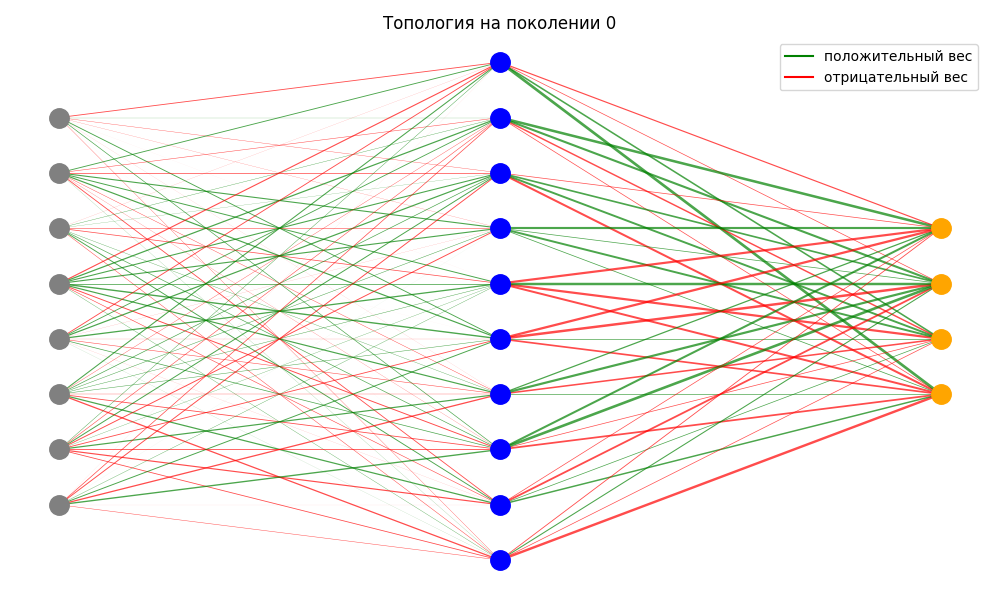
\includegraphics[width=0.7\textwidth]{images/topologies/topology_gen_0.png}
	\caption{Визуализация нейросети на 0-м поколении}
	\label{fig:struct_screenshot}
\end{figure}

\begin{figure}[H]
	\centering
	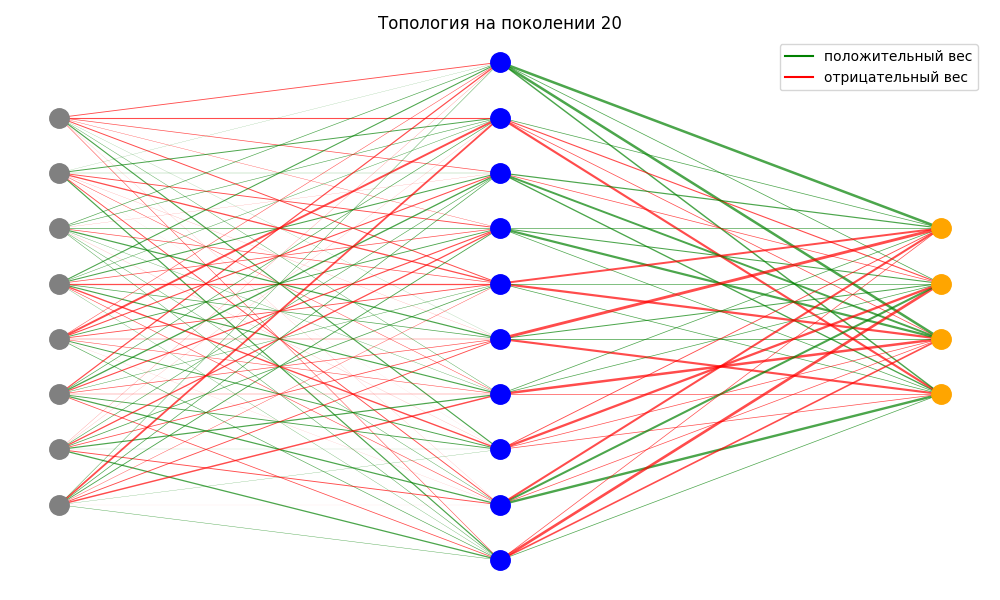
\includegraphics[width=0.7\textwidth]{images/topologies/topology_gen_20.png}
	\caption{Визуализация нейросети на 20-м поколении}
	\label{fig:struct_screenshot}
\end{figure}

\begin{figure}[H]
	\centering
	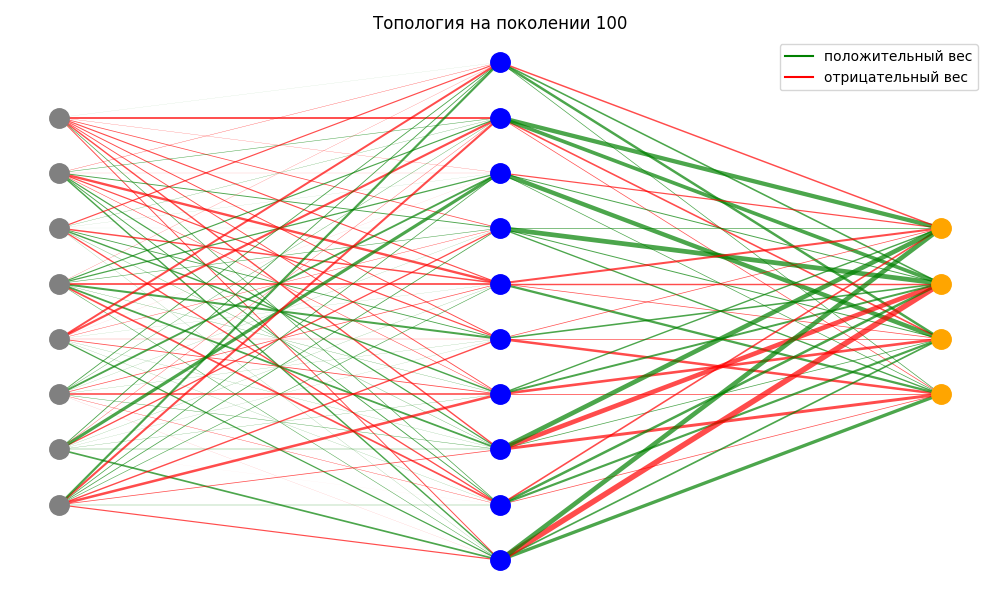
\includegraphics[width=0.7\textwidth]{images/topologies/topology_gen_100.png}
	\caption{Визуализация нейросети на 100-м поколении}
	\label{fig:struct_screenshot}
\end{figure}

\begin{figure}[H]
	\centering
	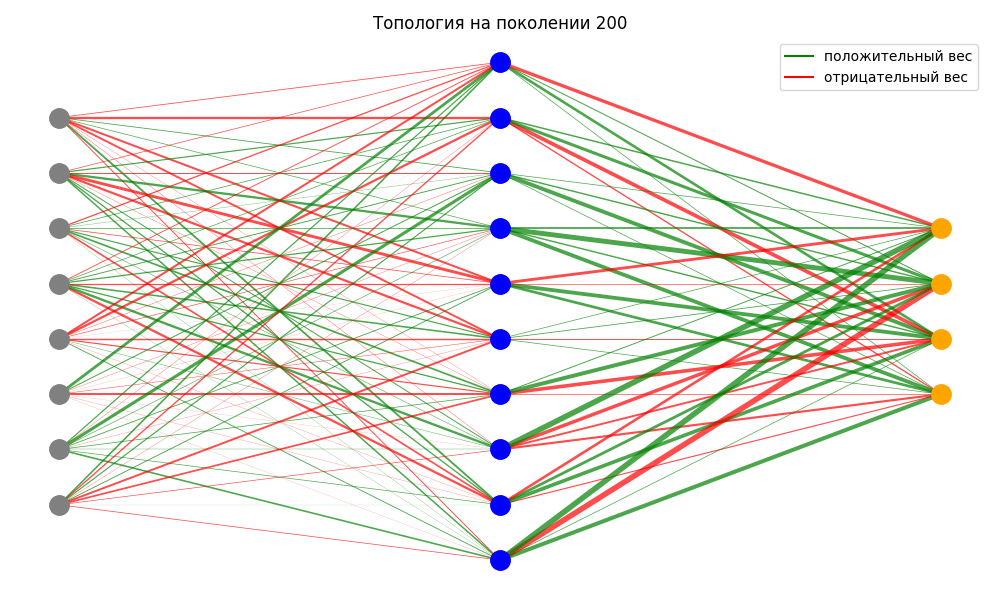
\includegraphics[width=0.7\textwidth]{images/topologies/topology_gen_200.png}
	\caption{Визуализация нейросети на 200-м поколении}
	\label{fig:struct_screenshot}
\end{figure}

\begin{figure}[H]
	\centering
	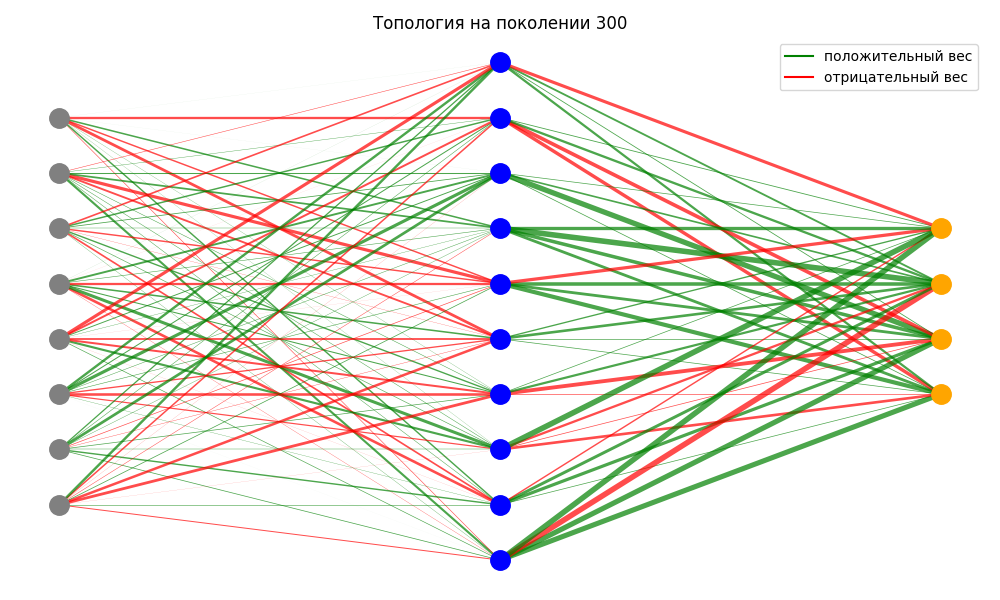
\includegraphics[width=0.7\textwidth]{images/topologies/topology_gen_300.png}
	\caption{Визуализация нейросети на 300-м поколении}
	\label{fig:struct_screenshot}
\end{figure}

\subsection{График изменения целевой метрики}

В процессе обучения после каждой оценки сохраняется значение метрики $R_{\text{avg}}$ (среднего вознаграждения за эпизод). По окончании обучения строится график, демонстрирующий изменение этой метрики по мере прохождения поколений.

\begin{itemize}
    \item В общем случае, значение $R_{\text{avg}}$ демонстрирует \textbf{рост во времени}, что указывает на адаптацию агента и улучшение его поведения.
    \item Однако иногда наблюдаются \textbf{резкие локальные падения} метрики — это следствие \textbf{неудачных мутаций}, временно ухудшающих поведение агента.
    \item Благодаря отбору и кумулятивному эффекту успешных мутаций, система продолжает развиваться и метрика стабилизируется на высоком уровне.
\end{itemize}

\begin{figure}[H]
	\centering
	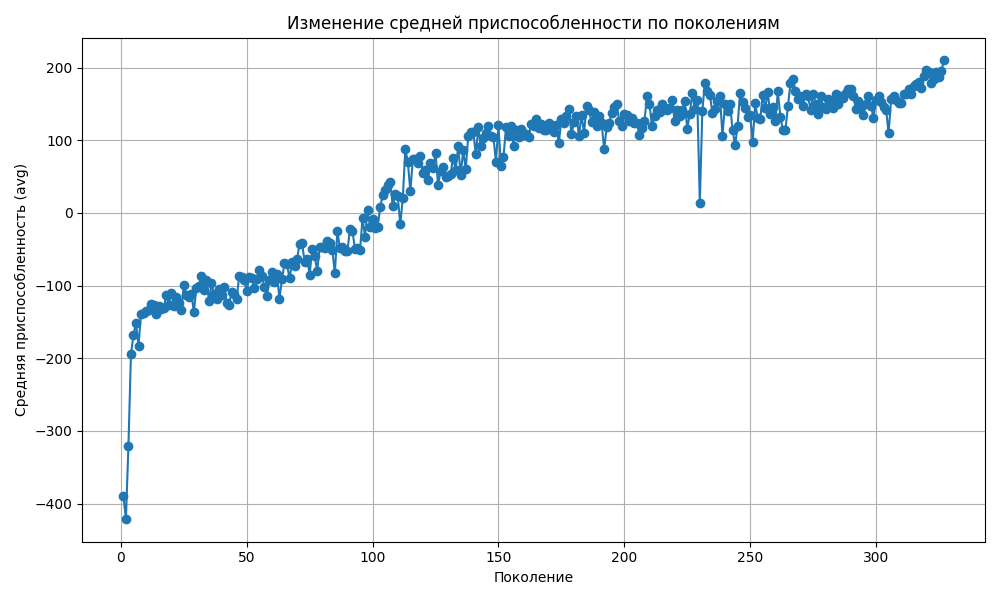
\includegraphics[width=0.7\textwidth]{images/avg_fitness_graph.png}
	\caption{График изменения $R_{\text{avg}}$ на протяжении обучения}
	\label{fig:struct_screenshot}
\end{figure}

\subsection{Интерпретация наблюдений}

Эти визуализации позволяют не только количественно оценить прогресс обучения, но и качественно проанализировать структуру сформировавшейся нейросети:
\begin{itemize}
    \item Структура сети становится более организованной, веса перераспределяются в пользу наиболее эффективных связей.
    \item Мутации выступают как источник вариативности, способный как улучшить, так и ухудшить поведение, но за счёт естественного отбора плохие изменения отбрасываются.
\end{itemize}

Таким образом, визуализация предоставляет важный инструмент для понимания динамики обучения агента, выявления закономерностей в формировании связей и анализа устойчивости процесса оптимизации.



\newpage


\section{Результаты обучения модели}

После завершения процесса эволюционного обучения можно сделать вывод о его успешности. Изначально агент демонстрировал крайне неэффективное поведение: среднее значение целевой метрики $R_{\text{avg}}$ составляло около $-400$, что указывало на частые аварийные посадки и полную неспособность управлять движением.

Однако по мере эволюции модели ситуация кардинально изменилась. На момент принудительной остановки обучения (на 200-м поколении) значение $R_{\text{avg}}$ достигло положительного уровня и стабилизировалось, что свидетельствует о сформировавшихся устойчивых стратегиях управления.

\subsection{Анализ поведения после обучения}

Агент начал демонстрировать следующие положительные черты поведения:
\begin{itemize}
    \item \textbf{Мягкая посадка} — вместо резкого столкновения с поверхностью, как это было на начальных этапах, агент плавно снижает скорость и корректирует вертикальное ускорение.
    
    \item \textbf{Точное позиционирование} — наблюдается способность удерживать корабль вблизи центра посадочной площадки, избегая отклонений влево или вправо.
    
    \item \textbf{Сбалансированное использование двигателей} — агент научился включать основной и боковые двигатели в нужные моменты, избегая лишнего расхода топлива и дестабилизации.
\end{itemize}

\subsection{Общие выводы}

Таким образом, в процессе обучения нейросеть смогла выработать стратегию, соответствующую целевой задаче. Поведение стало:
\begin{itemize}
    \item адаптивным;
    \item устойчивым;
    \item энергоэффективным;
    \item безопасным с точки зрения посадки.
\end{itemize}

Это доказывает, что применённый метод эволюционного обучения способен обучить агента эффективному управлению даже в условиях высокой неопределённости и сложной динамики.

\begin{center}
    \textit{[Рисунок 3: Пример успешной посадки после завершения обучения]}
\end{center}


\begin{figure}[H]
	\centering
	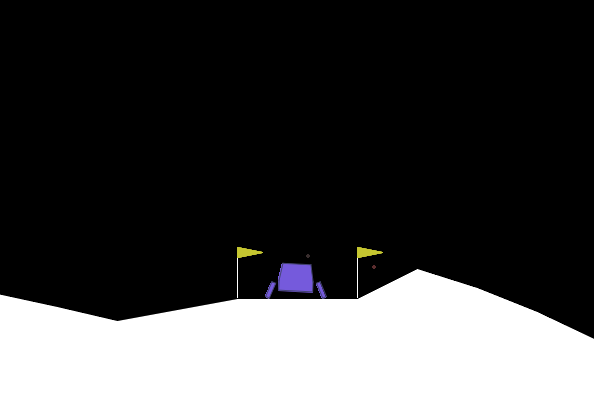
\includegraphics[width=0.7\textwidth]{images/successful_landing.png}
	\caption{Пример успешной посадки после завершения обучения}
	\label{fig:struct_screenshot}
\end{figure}


\newpage
\section*{Заключение}

В рамках лабораторной работы была реализована и протестирована система эволюционного обучения нейронной сети, управляющей агентом в среде \texttt{LunarLanderContinuous-v3}. Основной целью являлось формирование устойчивой стратегии посадки лунного модуля при помощи методов безградиентной оптимизации.

В процессе экспериментов был проведён сбор и анализ ключевых метрик, включая среднее суммарное вознаграждение ($R_{\text{avg}}$), визуализация архитектуры нейросети и динамики её весов, а также отслеживание общей динамики процесса обучения. На ранних этапах агент демонстрировал неэффективное поведение, что отражалось в отрицательных значениях метрики ($R_{\text{avg}} \approx -400$). Однако в ходе обучения наблюдался устойчивый рост среднего вознаграждения, что свидетельствовало о постепенном формировании корректной стратегии управления.

После завершения обучения агент научился выполнять мягкие посадки, точно позиционироваться в пределах посадочной зоны, избегать избыточного расхода топлива и поддерживать устойчивое вертикальное положение. Это подтверждает, что разработанная система успешно справляется с поставленной задачей и способна обучать агентов эффективному поведению в условиях непрерывного управления.

Полученные результаты демонстрируют потенциал эволюционных алгоритмов при решении задач управления в симулированных физических средах и открывают возможности для дальнейших исследований в области обучения с подкреплением без градиентной информации.


\newpage
% Список литературы
\section*{Список использованной литературы}
\begin{enumerate}
    \item Лекция 7. Алгоритмы ESP и H-ESP. Томский политехнический университет, 2025.
    \item Such F. P., Madhavan V., Conti E. [и др.]. Deep Neuroevolution: Genetic Algorithms Are a Competitive Alternative for Training Deep Neural Networks for Reinforcement Learning // arXiv preprint arXiv:1712.06567. — 2017. — URL: \url{https://arxiv.org/abs/1712.06567} (дата обращения: 07.06.2025). 
\end{enumerate}

\end{document}